\section{Models}

This section is dedicated to the two different models that have been used to map out our simulation. Firstly, we have used the MoSCoW method of prioritisation to decide on what must, should, could and will not be in our simulation. Secondly, we have created a flowchart over the simulation to more effectively communicate the structure of the program. The goal of using these two models is to create an overview of and guideline to the program.

\subsection{MoSCoW Method}

The MoSCoW method is used to make decisions on what elements must, should, could and will not be included in a product. The elements that must be included are elements that is absolutely necessary for the product to function at all. These therefore have the highest possible priority. The further right in the diagram the less necessary the element is to the core function of the product, these however might add more details which can make the product more accurate. The elements that will not be included, might be elements taken out due to time constraints in the project. They could also be elements that are unnecessary or not in focus in our project.

\begin{center}

\begin{tabularx}{0.9\textwidth} { 
  | >{\raggedright\arraybackslash}X 
  | >{\raggedright\arraybackslash}X 
  | >{\raggedright\arraybackslash}X
  | >{\raggedright\arraybackslash}X| }

 \hline
 \multicolumn{4}{|c|}{Simulation} \\
 \hline
  Must &  Should & Could & Will not \\
 \hline
   -Contact tracing \newline -Static R-value \newline -Time frame \newline -Medical states \newline -Population 
 
 & -Incubation \newline -Hospital Cap. \newline -Demographics \newline -Severity and death
 
 & -Fluid R-value \newline -Immune response period \newline -Other preventive measures
 
 & -Mutations \newline -Culture \newline -Living conditions \newline -Climate \newline -Misinformation \\
 
\hline
\end{tabularx}

\end{center}

The choices in the must-have column reflect what has been deemed absolutely necessary to make a useful simulation. If these factors are excluded, the simulation simply wouldn't work. The factors in this column are simply put the values from the SIR-model \ref{sec: SIR-based simulation} and contact tracing, which is the focus of our project. The population is included here because there needs to be a population of people to infect so the simulation can progress. The R-value represents the average amount of people an infected person will infect in the period they are sick. It has been set as a static value here to simplify it.

The time frame is necessary since the simulation needs to run for a certain amount of time to output several, different values. The length of this time frame directly affects whether the results will give an accurate representation of reality, since a short time frame might not show when the infection dies out, which can give unusable results. 

In a similar vein, different medical states are important so a person can be determined to be susceptible to, infected by or recovered from COVID-19. Lastly, contact tracing has been deemed as a must-have because it is a requirement in the chosen project.

The different factors in the should-have column have been selected because they are important for the simulation to be more accurate, but not necessary for the simulation to function. Factors like hospital capacity, demographics and severity would create a more lifelike simulation, and therefore, they have been included in this column. Incubation has been included to delay infection chance, as is also the case with real-world data.
 
The factors in the could-have column are elements that might make the simulation even more precise and realistic, but not deemed necessary for the simulation to run well. The R-value, which has been set as static in the must-have column would most likely change as a result of several variables' influence. Therefore, a static R-value is considered a must-have, where an R-value that is interdependent on other variables is considered a could-have.

Occurrences of people getting infected twice or more with COVID-19 suggest that an individual has an immune response period after which they would be able to get infected again. As there are varying opinions on re-infection chance among scholars at the time of writing \citep{malkov_simulation_2020}, this was given a lower priority. Lastly, other preventive measures (as mentioned in subsection \ref{sec: preventive measure}) will make for a more accurate representation of contact tracing's effect on prevention, but is not necessary to gain an insight into contact tracing's effect on its own.

Lastly, the factors placed in the will-not-have column are elements that are either beyond the expertise of the group or deemed irrelevant for the simulation. For instance, mutations of the virus, while intriguing, would influence the very basis of the study, as the study is focused on COVID-19. Likewise, including misinformation (\say{fake news}) as a variable in the program arguably makes for a more precise simulation, but misinformation is not easily implemented into a program. The remaining factors in this column (culture, living conditions and climate) have been left out of the program because of time constraints and minimal relevance for the project.

After getting a better understanding of what elements are essential for our simulation through the use of MoSCoW, we were able to start designing our program through flowcharts.

\subsection{Flowcharts} \label{sub: flowcharts}
We have used flowcharts to get a more thorough understanding of how our program will work before we actually make it. The flowcharts included below are the newest version. Our first draft of a flowchart for the most basic version of our simulation can be seen in appendix \vref{Appendix:FirstFlowchart}. Below is a walk-through of the finished flowchart, which most accurately resembles the source code. The flowchart has been divided into two parts for readability.

\begin{figure}[H]
  \centering
  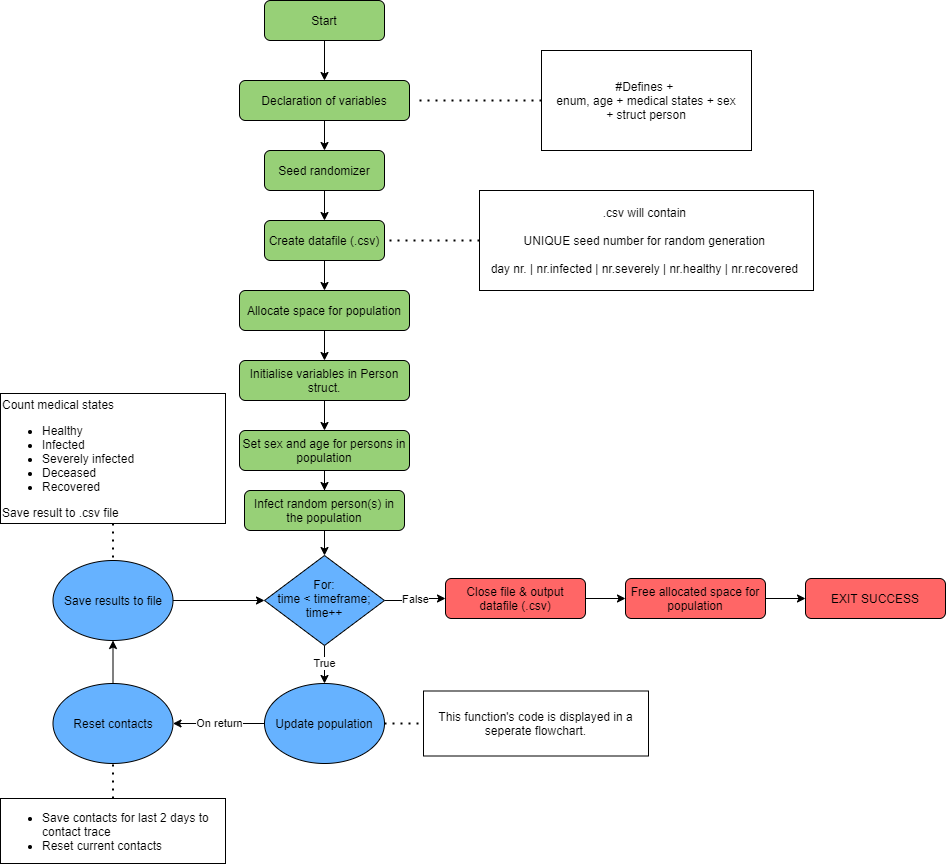
\includegraphics[width=\textwidth]{0_billeder/Part1Flowchart.png}
  \caption{Part 1 of the flowchart, the core program.}
  \label{fig:Part1Flow}
\end{figure}

In the first part seen in figure \ref{fig:Part1Flow} is the core part of our program, with the declaration/initialisation phase(marked in green), the main loop of our program(marked in blue) as well as the end of the program when the main loop is exited(marked in red).

The main loop includes functions that update the population, resets the contacts which the infected has been in contact with and saves relevant data to an output file. The update population function will be described further below in figure \vref{fig:Part2Flow}, since its the most important function. 

\begin{figure}[H]
  \centering
  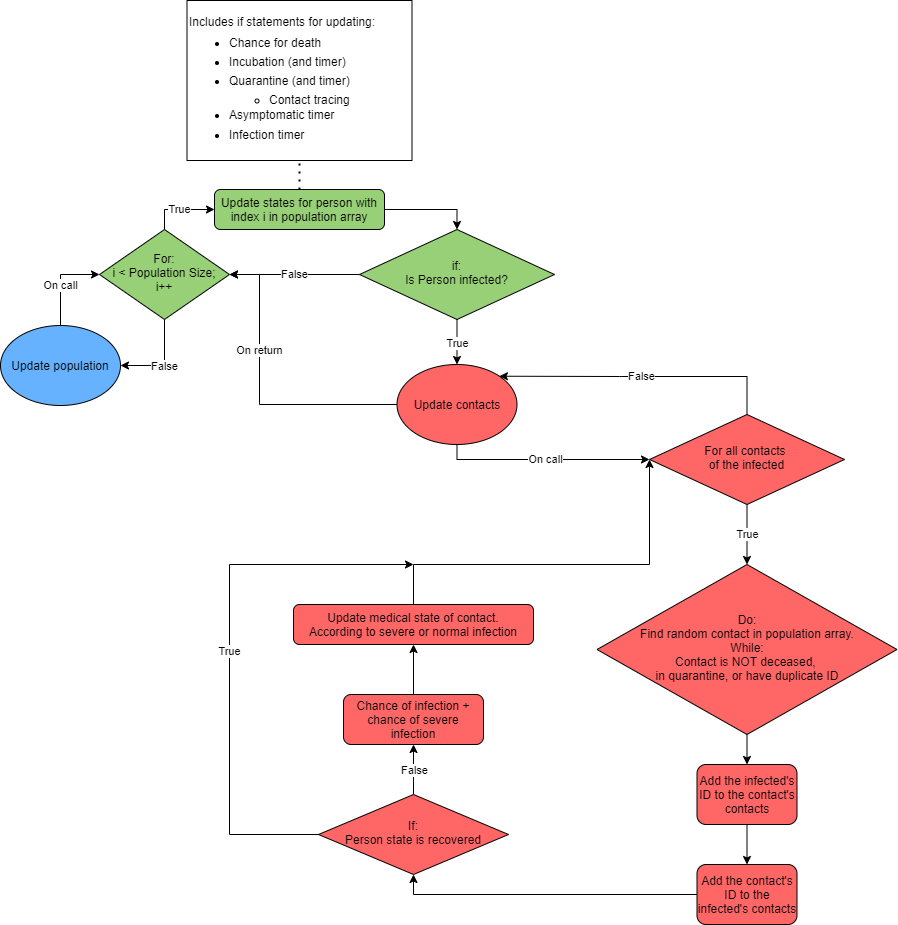
\includegraphics[width=\textwidth]{0_billeder/Part2Flowchart.png}
  \caption{Part 2 of the flowchart, extended program.}
  \label{fig:Part2Flow}
\end{figure}

As seen in figure \vref{fig:Part2Flow}, it continues from the function that updates population (in blue, leading to green). Within this function, the program runs through the entire population to not only check whether the given person is infected, but also to run through their contacts (in red). If the person is not infected, a new person is checked. However, if the person is infected, it continues to the next function call (in red).

The function that updates contacts checks through all contacts of the person. If the contact is not deceased, in quarantine or has already been checked, the contact and person exchange ID's, so they can not be re-selected as a contact until the contacts are reset. 
If the contact is susceptible, there is a chance they can become infected, after which their medical state is updated accordingly. Update contacts runs until the infected has no more contacts, after which the program loops out of the function.